\begin{figure}[H]
  \centering
  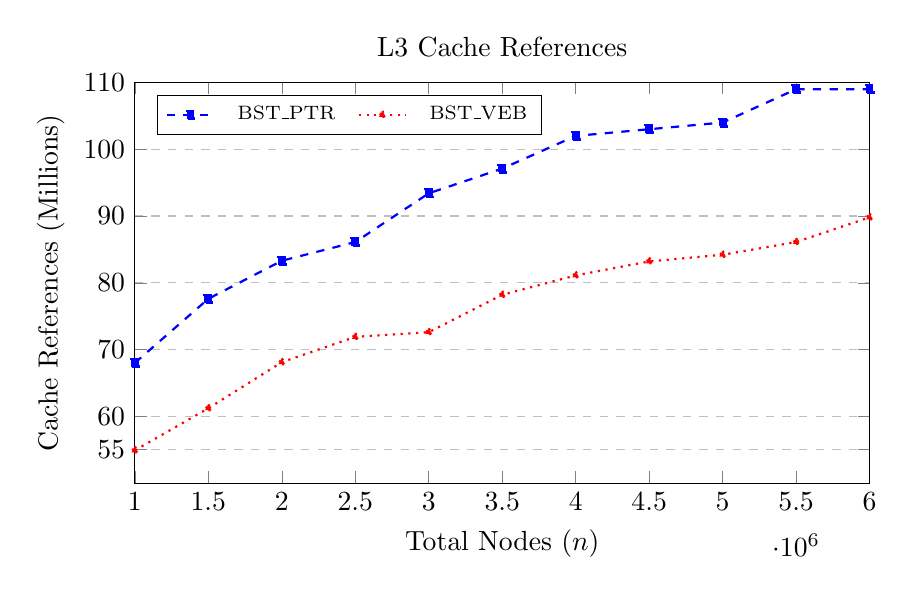
\begin{tikzpicture}
    \begin{axis}[
        title={L3 Cache References},
        xlabel={Total Nodes ($n$)},
        ylabel={Cache References (Millions)},
        width=0.9\textwidth,
        height=0.55\textwidth,
        xmin=1000000, xmax=6000000,
        ymin=5.0e7, ymax=1.1e8,
        ymajorgrids,
        grid style=dashed,
        legend columns=2,
        legend pos=north west,
        legend style={font=\scriptsize, column sep=6pt},
        scaled y ticks=false,
        ytick={5.5e7, 6e7, 7e7, 8e7, 9e7, 1e8, 1.1e8},
        yticklabels={55, 60, 70, 80, 90, 100, 110}
    ]

    \addplot+[blue, thick, dashed, mark=square*, mark options={scale=.7,fill=blue}]
      coordinates {
        (1000000,6.80e7) (1500000,7.76e7) (2000000,8.33e7) (2500000,8.61e7)
        (3000000,9.34e7) (3500000,9.71e7) (4000000,1.02e8) (4500000,1.03e8)
        (5000000,1.04e8) (5500000,1.09e8) (6000000,1.09e8)
      };
    \addlegendentry{BST\_PTR}

    \addplot+[red, thick, dotted, mark=triangle*, mark options={scale=.7,fill=red}]
      coordinates {
        (1000000,5.49e7) (1500000,6.12e7) (2000000,6.81e7) (2500000,7.19e7)
        (3000000,7.26e7) (3500000,7.82e7) (4000000,8.11e7) (4500000,8.32e7)
        (5000000,8.42e7) (5500000,8.61e7) (6000000,8.98e7)
      };
    \addlegendentry{BST\_VEB}

    \end{axis}
  \end{tikzpicture}
  \caption{L3 Cache references in millions as a function of total nodes for $q=1000000$ lookups for the pointer-based (\texttt{BST\_PTR}) and Van Emde Boas (\texttt{BST\_VEB}) implementations.}
  \label{fig:l3refs}
\end{figure}
